\section{Quantitation of the Spurious Response}
In this work, a continuous--time signal/function is denoted by lowercase letters, for example, $u\left(t\right)$. It's duality in the frequency domain (via Fourier transform) is denoted with a overhead hat, for example, $\hat{u}\left(\omega\right)$ or $\hat{u}\left(f\right)$. A discrete--time signal is denoted by square brackets, for example, $u[n]$. The counterpart in the frequency domain (via the discrete Fourier transform) is denoted by the uppercase letter, for example, $U[n]$. It can alternatively be approximated by sampling $\hat{u}\left(\omega\right)$ or $\hat{u}\left(f\right)$. The conversion between angular frequency $w$ and frequency $f$ is done implicitly.
\subsection{Linear Interpolation}
For the ease of discussion, let sampling interval be the multiple of time step size and let the ratio be $L$, which is an integer. It is then equivalent to upsample the input seismogram by the same ratio $L$. If the sampling rate/frequency of the original seismogram is $f_s$, then the upsampled signal has a sampling rate of $Lf_s$. Extra attention shall be paid to the original Nyquist frequency $f_s/2$ since anything above it cannot be reliably reconstructed. For a discrete--time signal $p[n]$, a typical upsampling operation with upsampling factor $L$ consists of two steps \citep{Oppenheim2010}:
\begin{enumerate}
\item Insert $L-1$ zeros between each pair of adjacent samples in $p[n]$, resulting in a new signal $p_e[n]$ which can be formally defined as
\begin{gather}
p_e[n]=\left\{
\begin{array}{ll}
p[n/L],&n=0,~L,~2L,~3L,~\cdots,\\
0,&\text{otherwise}.
\end{array}
\right.
\end{gather}
This is known as an expander, and is often denoted by $\uparrow{}L$ such that $p_e[n]=[\uparrow{}L]p[n]$.
\item Apply a low--pass filter with kernel $g[n]$ on $p_e[n]$ via convolution. The linear interpolation corresponds to the following kernel.
\begin{gather}
g[n]=\left\{
\begin{array}{ll}
1-\abs{n}/L,&\abs{n}\leqslant{}L-1,\\
0,&\text{otherwise}.
\end{array}
\right.
\end{gather}
The convoluted/interpolated/filtered signal is denoted as $p_i[n]$. In this work, different kernels will be discussed.
\end{enumerate}

Since the extended discrete signal $p_e[n]$ is $p[n]$ with additional zero samples, once the upsampling factor $L$ is chosen, $p[n]$ can be converted to $p_e[n]$ and vice versa. We focus on the properties of $p_e[n]$.

The bare $p_e[n]$ without applying any filters contains spectral images, that is, extra copies of the original spectrum $f\in[0,~f_s/2]$ in additional frequency domain $f\in[f_s/2,~Lf_s/2]$. For example, consider the sinusoid
\begin{gather}
u(t)=\sin\left(2\pi{}f_0t\right),
\end{gather}
with the frequency $f_0=\dfrac{\omega_0}{2\pi}$ chosen to be \SI{25}{\hertz}, a typical upper bound of seismograph. Assume this continuous--time signal is sampled at a rate of $f_s=\SI{200}{\hertz}$, the discrete--time signal $p[n]$ can be depicted in \figref{fig:original}.
\begin{figure}[htb!]
\centering
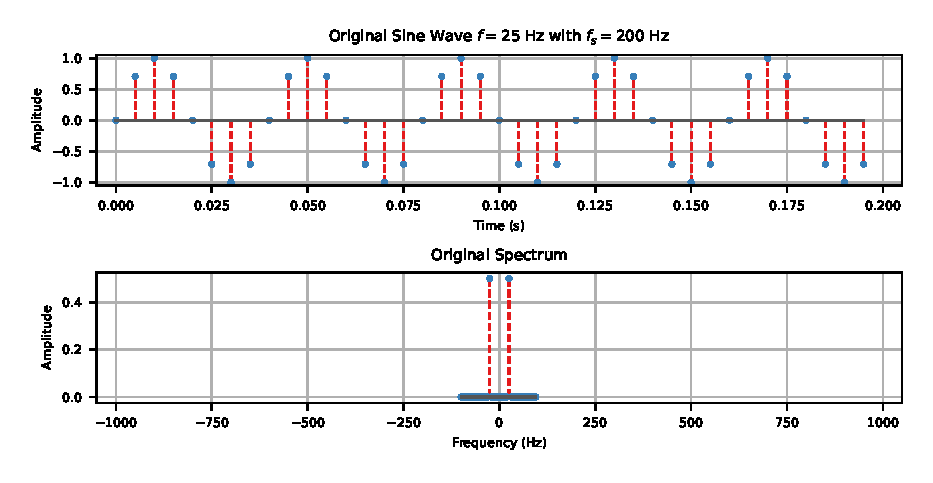
\includegraphics{PIC/PureSineOrigin}
\caption{original sine wave in time domain and frequency domain}\label{fig:original}
\end{figure}
The corresponding Nyquist frequency is $f_s/2=\SI{100}{\hertz}$, thus, the frequency ranges from \SI{-100}{\hertz} to \SI{100}{\hertz} (negative part not shown with amplitude properly scaled).

By choosing an upsampling factor $L=10$, the extended signal $p_e[n]$ (zero--stuffed) can be illustrated as in \figref{fig:extended}.
\begin{figure}[htb!]
\centering
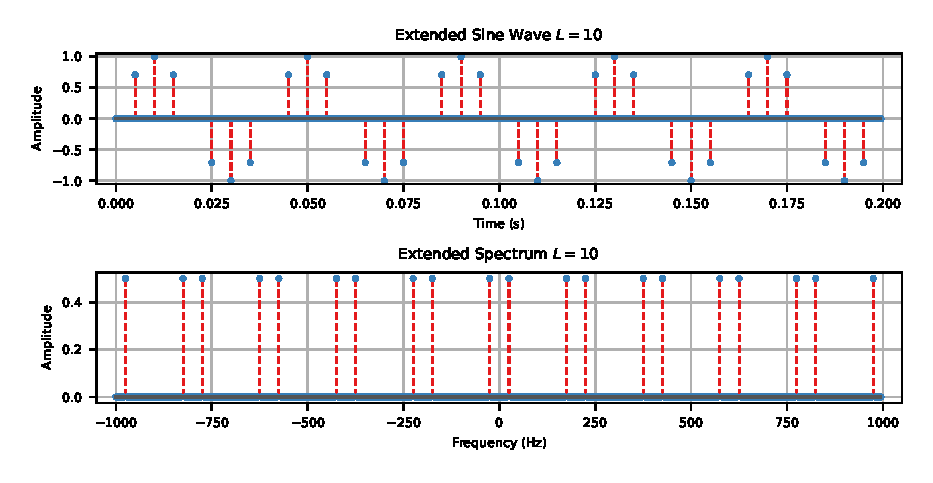
\includegraphics{PIC/PureSineExtended}
\caption{zero--stuffed sine wave in time domain and frequency domain}\label{fig:extended}
\end{figure}
The Nyquist frequency of $p_e[n]$ is $10\times\SI{100}{\hertz}=\SI{1000}{\hertz}$, the original component at $\SI{25}{\hertz}$ is copied in the additional frequency domain ranging from \SI{100}{\hertz} to \SI{1000}{\hertz}.

The linear interpolation (triangular window) for $L=10$ can be constructed as
\begin{gather}
g[n]=0.1\times\begin{bmatrix}
1&2&3&\cdots&10&\cdots&3&2&1
\end{bmatrix},
\end{gather}
its frequency response $G[n]$ can be obtained via the discrete Fourier transform, which is shown in \figref{fig:tri_window}.
\begin{figure}[htb!]
\centering
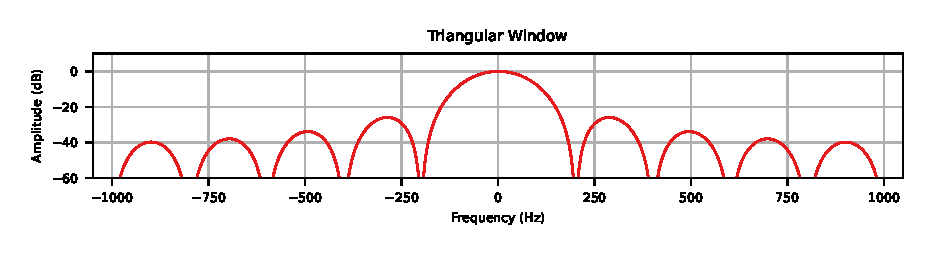
\includegraphics{PIC/TriangularWindow}
\caption{triangular window in frequency domain}\label{fig:tri_window}
\end{figure}
The analytical expression can be obtained via convoluting two rectangular signals, which gives
\begin{gather}\label{eq:tri_kernel}
\hat{g}\left(f\right)=\text{sinc}^2\left(\dfrac{2f}{f_s}\right).
\end{gather}

By the convolution theorem, the upsampled signal can be obtained by either performing the convolution in time domain or multiplication in frequency domain.
\begin{figure}[htb!]
\centering
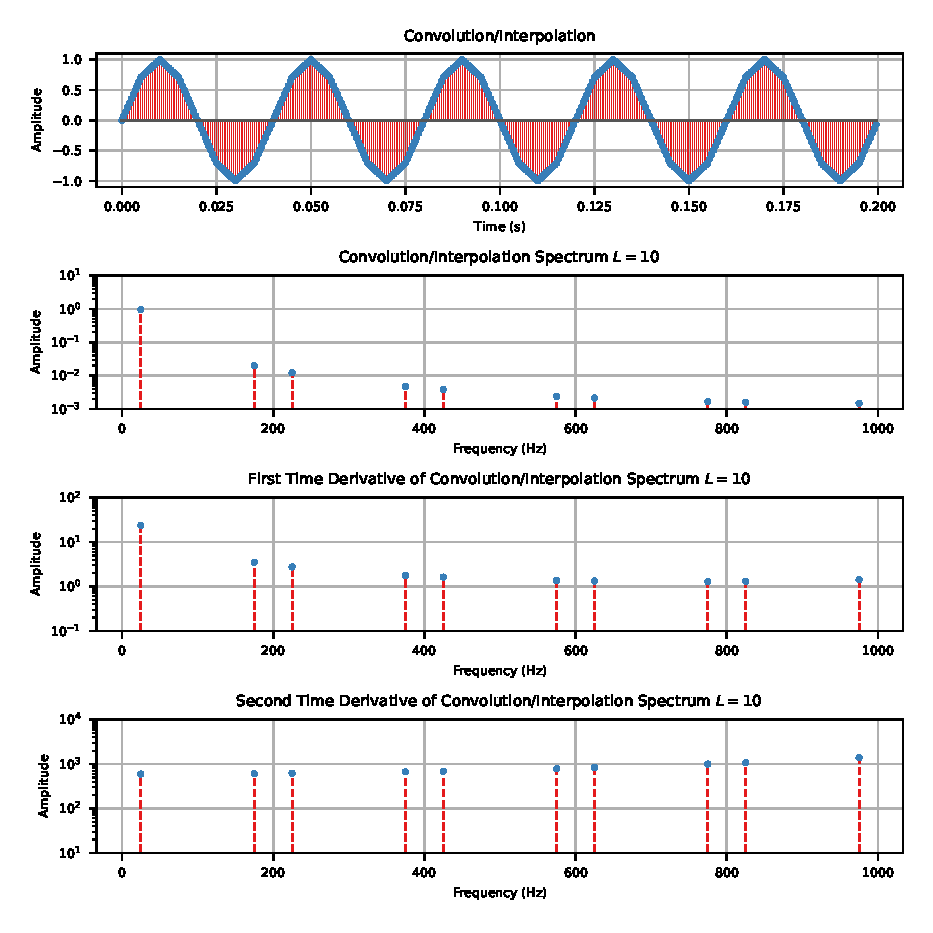
\includegraphics{PIC/Convolution}
\caption{interpolated sine wave in time domain and frequency domain}\label{fig:interpolated}
\end{figure}
\figref{fig:interpolated} shows the interpolated signal in both time domain and frequency domain. Due to the high side lobe level (around \SI{-26}{\decibel} of the first side lobe) of the triangular window, the spectral images in $p_i[n]$ between \SI{100}{\hertz} and \SI{1000}{\hertz} are seemingly attenuated, but their magnitudes are relatively large. The interpolated signal is used to formulate external load that is used in dynamic analysis.
\subsection{Oscillator System}
To investigate how the partially attenuated images would affect the response of oscillator systems, consider a single degree of freedom mass--spring--dashpot linear system under harmonic load. The equation of motion can be written as
\begin{gather}
ma\left(t\right)+cv\left(t\right)+ku\left(t\right)=p\left(t\right),
\end{gather}
with $p\left(t\right)=p_0\sin\left(2\pi{}ft\right)$ where $p_0$ is the amplitude of the harmonic, and its angular frequency is $\omega=2\pi{}f$.

Duhamel's integral shows the solution to this system can be expressed as
\begin{gather}\label{eq:duhamel}
u\left(t\right)=\int_{0}^{t}p\left(\tau\right)h\left(t-\tau\right)\md{\tau},
\end{gather}
with the fundamental solution
\begin{gather}
h\left(t\right)=\dfrac{1}{m\omega_d}\exp\left(-\zeta\omega_nt\right)\sin\left(\omega_dt\right),
\end{gather}
where $m$ is the mass, $c$ is the damping coefficient, $k$ is the stiffness, $\omega_n=\sqrt{\dfrac{k}{m}}$ is the natural frequency of the system, $\zeta=\dfrac{c}{2\sqrt{mk}}$ is the damping ratio, $\omega_d=\omega_n\sqrt{1-\zeta^2}$ is the damped frequency. The following discussion is confined within underdamped cases ($\zeta<1$).

\eqsref{eq:duhamel} can be conveniently evaluated in the frequency domain via unilateral Laplace transform \citep[see, e.g.,][]{Lee1990}, such that
\begin{gather}
\hat{u}\left(\omega\right)=\mathscr{L}\left\{u\left(t\right)\right\}=\mathscr{L}\left\{p\left(t\right)\right\}\cdot\mathscr{L}\left\{h\left(t\right)\right\}=\hat{p}\left(\omega\right)\cdot\hat{h}\left(\omega\right),
\end{gather}
with
\begin{gather}\label{eq:analytical_transfer}
\hat{h}\left(\omega\right)=\dfrac{1}{k}\dfrac{1}{\left(1-\eta^2\right)+i\left(2\zeta\eta\right)},\qquad\eta=\dfrac{\omega}{\omega_n}.
\end{gather}

The velocity/acceleration spectrum can be obtained by differentiating $\hat{u}\left(\omega\right)$,
\begin{gather}
\hat{v}\left(\omega\right)=i\omega\cdot{}\hat{u}\left(\omega\right)=i\omega\cdot{}\hat{p}\left(\omega\right)\cdot\hat{h}\left(\omega\right),\\
\hat{a}\left(\omega\right)=i\omega\cdot{}\hat{v}\left(\omega\right)=-\omega^2\cdot{}\hat{p}\left(\omega\right)\cdot\hat{h}\left(\omega\right).
\end{gather}
\subsubsection{Damping Force}
If the damping force is denoted by $F_v$, then it is possible to derive that
\begin{gather}
\hat{F_v}\left(\omega\right)=\mathscr{L}\left\{F_v\left(t\right)\right\}=c\cdot{}\hat{v}\left(\omega\right)=c\cdot{}i\omega\cdot{}\hat{p}\left(\omega\right)\cdot\hat{h}\left(\omega\right).
\end{gather}
We further denote
\begin{gather}
\hat{k_v}\left(\omega\right)=ic\omega\cdot\hat{h}\left(\omega\right),
\end{gather}
which links external load spectrum $\hat{p}\left(\omega\right)$ to the damping force spectrum $\hat{F_v}\left(\omega\right)$.

Now consider three different types of damping.
\paragraph{Constant Damping}
Let $c$ (and $\zeta$) be a constant, then
\begin{gather}\label{eq:damping_constant}
\hat{k_v}\left(\omega\right)=\dfrac{i\left(2\zeta\eta\right)}{\left(1-\eta^2\right)+i\left(2\zeta\eta\right)}.
\end{gather}
\paragraph{Mass Proportional Damping}
Let $c$ be proportional to mass such that $c=2a_0m$, then
\begin{gather}
\zeta=\dfrac{2a_0m}{2\sqrt{mk}}=\dfrac{a_0}{\omega_n},\qquad
\zeta\eta=\dfrac{a_0\omega}{\omega_n^2},
\end{gather}
so that
\begin{gather}\label{eq:damping_mass}
\hat{k_v}\left(\omega\right)=\dfrac{i\left(2a_0\omega\right)}{\left(\omega_n^2-\omega^2\right)+i\left(2a_0\omega\right)}.
\end{gather}
\paragraph{Stiffness Proportional Damping}
Let $c$ be proportional to stiffness such that $c=2a_1k$, then
\begin{gather}
\zeta=\dfrac{2a_1k}{2\sqrt{mk}}=a_1\omega_n,\qquad
\zeta\eta=a_1\omega,
\end{gather}
so that
\begin{gather}\label{eq:damping_stiffness}
\hat{k_v}\left(\omega\right)=\dfrac{i\left(2a_1\omega\right)}{\left(1-\eta^2\right)+i\left(2a_1\omega\right)}.
\end{gather}

It can be noticed that all three expressions of $\hat{k_v}\left(\omega\right)$ possess a similar form
\begin{gather}\label{eq:general_damping_force}
\hat{k_v}\left(\omega\right)=\dfrac{iA}{B+iA},
\end{gather}
and $B=0$ when $\omega=\omega_n$, where the maximum magnitude \num{1} is achieved. At this exact point, the magnitude of damping force component simply equals that of the external load component. With that said, although damping ratio either decays to zero asymptotically (mass proportional) or grows to infinity (stiffness proportional), the corresponding damping force is bounded, the maximum of which is dependent of the magnitude of external load at the target frequency. The magnitude distribution of $\hat{k_v}\left(\omega\right)$ in frequency domain can be computed and illustrated in \figref{fig:constant_damping}, \figref{fig:k_proportional} and \figref{fig:m_proportional}.
\begin{figure}[htb!]
\centering
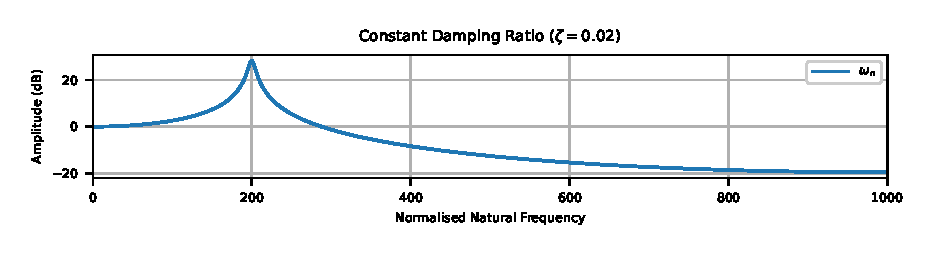
\includegraphics{PIC/ConstantProportional2000}
\caption{fundamental solution with constant damping}\label{fig:constant_damping}
\includegraphics{PIC/StiffnessProportional10}
\caption{fundamental solution with stiffness proportional damping}\label{fig:k_proportional}
\includegraphics{PIC/MassProportional500000}
\caption{fundamental solution with mass proportional damping}\label{fig:m_proportional}
\end{figure}

Since the external load $p\left(t\right)$ would be discretised for numerical analysis, it is possible to move the interpolation filter $\hat{g}\left(f\right)$ to $\hat{k_v}\left(f\right)$, we further denote the product by
\begin{gather}
\hat{m_v}\left(f\right)=\hat{g}\left(f\right)\cdot\hat{k_v}\left(f\right),
\end{gather}
such that
\begin{gather}
\hat{F_v}\left(f\right)=\hat{p_e}\left(f\right)\cdot\hat{m_v}\left(f\right),
\end{gather}
where $\hat{p_e}\left(f\right)$ is the spectrum of extended (zero--stuffed) external load that possesses identical magnitude at imaging frequencies, see \figref{fig:extended}.

One can plot the magnitude of $\hat{m_v}\left(f\right)$ in frequency domain by choosing different natural frequency $f_n$ and damping model parameters. One example is given in \figref{fig:k_proportional_damping}.
\begin{figure}[htb!]
\centering
\includegraphics{PIC/StiffnessDampingForce200-10}
\caption{magnitude of $\hat{m_v}\left(f\right)$ for $f_n=\SI{200}{\hertz}$ with $a_1=0.0001$}\label{fig:k_proportional_damping}
\end{figure}
If $p_e[n]$ and $F_v[n]$ are treated as input and output respectively, $\hat{m_v}\left(f\right)$ is then the corresponding transfer/kernel function.
The analytical expression of $\hat{m_v}\left(f\right)$ provides a conveniently tool to query the magnitude of damping force. For example, if the upsampled sine wave in \figref{fig:extended} is used as the external load, it has a \SI{25}{\hertz} component with a magnitude of \num{1}, then the damping force shall have the same component of a magnitude $1\times\num{3.03e-2}$. The factor \num{3.03e-2} is obtained by computing the magnitude of $\hat{m_v}\left(f\right)$ at $f=\SI{25}{\hertz}$. Similarly, the \SI{225}{\hertz} component shall have a magnitude of \num{8.91e-3}.
\subsubsection{Inertial Force}
Similarly, the inertial force can be derived as
\begin{gather}
\hat{F_a}\left(f\right)=\hat{p_e}\left(f\right)\cdot\hat{m_a}\left(f\right),\qquad
\hat{m_a}\left(f\right)=\hat{g}\left(f\right)\cdot\hat{k_a}\left(f\right),
\end{gather}
where
\begin{gather}\label{eq:inertial_force}
\hat{k_a}\left(\omega\right)=-m\omega^2\cdot\hat{h}\left(\omega\right)=\dfrac{-\eta^2}{\left(1-\eta^2\right)+i\left(2\zeta\eta\right)}.
\end{gather}
For stiffness/mass proportional damping, $\zeta$ takes the same expressions, viz., $a_1\omega_n$ and $a_0/\omega_n$, respectively.
\subsubsection{Remarks}
We derive the transfer functions $\hat{m_v}\left(f\right)$ and $\hat{m_a}\left(f\right)$ between the zero--stuffed input (external load) and the output (damping/inertial force) as follows.
\begin{gather}
\hat{m_v}\left(f\right)=\hat{g}\left(f\right)\cdot\hat{k_v}\left(f\right),\\
\hat{m_a}\left(f\right)=\hat{g}\left(f\right)\cdot\hat{k_a}\left(f\right).
\end{gather}
The filter kernel $\hat{g}\left(f\right)$ can take various forms, depending on the specific type of filters chosen. For linear interpolation (triangular window), it possesses the analytical expression as shown in \eqsref{eq:tri_kernel}. The terms $\hat{k_v}\left(f\right)$ and $\hat{k_a}\left(f\right)$ also takes various forms, as shown in \eqsref{eq:damping_constant}, \eqsref{eq:damping_mass}, \eqsref{eq:damping_stiffness} and \eqsref{eq:inertial_force}, depending on the type of damping used.

One can evaluate $\hat{m_v}\left(f\right)$ and $\hat{m_a}\left(f\right)$ over the whole frequency domain for different damping models and upsampling filters. Two example are given as follows.
\begin{figure}[htb!]
\centering
\begin{subfigure}{.48\textwidth}
\includegraphics{PIC/ConstantMapTri-2000}
\caption{damping case $\hat{m_v}\left(f\right)$}
\end{subfigure}
\begin{subfigure}{.48\textwidth}
\includegraphics{PIC/InertialMapTri-2000}
\caption{inertial case $\hat{m_a}\left(f\right)$}
\end{subfigure}
\caption{normalised damping/inertial force magnitude with constant damping ratio and triangular window}\label{fig:map_constant}
\end{figure}
\begin{figure}[htb!]
\centering
\begin{subfigure}{.48\textwidth}
\includegraphics{PIC/StiffnessMapTri-20}
\caption{damping case $\hat{m_v}\left(f\right)$}
\end{subfigure}
\begin{subfigure}{.48\textwidth}
\includegraphics{PIC/InertialStiffnessMapTri-20}
\caption{inertial case $\hat{m_a}\left(f\right)$}
\end{subfigure}
\caption{normalised damping/inertial force magnitude with stiffness proportional damping and triangular window}\label{fig:map_stiffness}
\end{figure}
In \figref{fig:map_constant}, the triangular window $L=10$ is chosen with a constant damping ratio $\zeta=\num{0.02}$. In \figref{fig:map_stiffness}, the triangular window $L=10$ is chosen with a stiffness proportional damping $a_1=\num{2e-4}$. In both examples, it is clearly seen that the undesired response at frequencies ranging from \SI{100}{\hertz} and \SI{1000}{\hertz} (that do not exist in the original signal, see \figref{fig:original}) is poorly attenuated. The magnitude of which is comparable to that of the original signal. Under certain circumstances (depending on the properties of the target system), numerical results of the corresponding analysis may be unreliable/unusable.
\subsection{A Preliminary Example}\label{sec:sdof_example}
The concept is best validated via a simple example. A single degree of freedom system is modelled with the following parameters.
\begin{gather}
f_n=200,\quad{}m=1,\quad{}k=4\pi^2f_n^2=\num{1.579e6},\quad{}a_1=\num{e-4},\quad{}c=2a_1k=\num{315.827},
\end{gather}
with the external load and time step size
\begin{gather}
p\left(t\right)=\sin\left(50\pi{}t\right),\quad\Delta{}t=\num{5e-4}.
\end{gather}
For comparison, the external load is provided in both forms: 1) sampled at \SI{200}{\hertz} and upsampled to \SI{2000}{\hertz} as shown in \figref{fig:interpolated}, and 2) analytically evaluated at each time point. The damping/inertial force history and its frequency components are shown in \figref{fig:sdof_force}.
\begin{figure}[htb!]
\centering
\includegraphics{PIC/InterpolationExample}
\caption{damping/inertial force history and spectrum of the SDOF system (transient solution included) using triangular widow and Newmark method with $\gamma=0.5$ and $\beta=0.25$}\label{fig:sdof_force}
\end{figure}
The interpolated external load results in significant overshoots (around \SI{50}{\percent} for damping force and around \SI{500}{\percent} for inertial force) due to significant components at \SI{175}{\hertz} and \SI{225}{\hertz}, which are not attenuated by the linear interpolation. The values agree with \figref{fig:k_proportional_damping}.

Given that numerical models inevitably contain high frequency modes due to, for example, finite element discretisation, the presence of constraints implemented via the penalty function method, under-integrated mass matrix or even lumped mass matrix with zero diagonals, the contribution of high frequency to damping/inertial force can be amplified significantly. It must be emphasised that according to \eqsref{eq:general_damping_force}, as long as damping is considered, no matter which type, the maximum possible magnitude of damping force of a specific frequency equals to that of the upsampled (after filtering) input (external load in this case). Furthermore, it is also independent of the magnitude of damping, small or large. In fact, a large damping ratio gives flat $\hat{k_v}\left(f\right)$, which reduces the difference between low frequency response and high frequency response. It is thus less likely to overshoot regarding damping force (only). It can also be concluded that, as long as the damping model is not point--based (for example, the Wilson--Penzien model, which only responds to selected frequency points), the system is \textbf{not} immune from spurious damping force. It is also evident from analytical expressions that as long as $m$ is not zero, inertial force would be affected by this type of spurious response.

In the case of multiple degrees of freedom (MDOF) system, depending on the distribution of natural frequencies and the components of the external load, as well as the upsampling ratio, it is possible that higher modes produce significant response due to, for example, being closer to imaging frequencies. The final numerical results may contain a considerably large portion of spurious response.
\section{Remedies and Recommendations}
As can be seen in \figref{fig:sdof_force}, using analytical expression for external load is clearly a solution that can fully suppress spurious response. However, this is not an option as the analytical expression of seismograph cannot be reconstructed easily.
\subsection{Low--pass Filters with Better Attenuation}
If the oscillator system is deemed as a filter system, it is evident that the fundamental cause of spurious force (output) is the high frequency noises in external load (input). A natural remedy is to suppress high frequency components as much as possible. In this regard, the linear interpolation is error prone. Other options are available.

Ideally, a low--pass filter that possesses high roll--off rate and low side lobe level can suppress the images caused by upsampling to the level that the corresponding spurious responses won't have a significant impact on final results, even after scaling up by a factor of $-\omega^2$.

In the following, we show a number of different windows in \figref{fig:nuttall_window}, \figref{fig:flattop_window}, \figref{fig:kaiser_window} and \figref{fig:cheb_window}, including the Blackman--Nuttall window, the flat top window, the Kaiser family and the Chebyshev family. Those are commonly used windows \citep{Oppenheim2010} in design of FIR filters. The number of bins is chosen to be $32L+1$ ($L=10$ in this work) to obtain a side lobe level around \SI{-100}{\decibel}.
\begin{figure}[htb!]
\centering
\includegraphics{PIC/Window-Nuttall}
\caption{Blackman--Nuttall window and the filtered signal}\label{fig:nuttall_window}
\end{figure}
\begin{figure}[htb!]
\centering
\includegraphics{PIC/Window-Flattop}
\caption{Flat top window and the filtered signal}\label{fig:flattop_window}
\end{figure}
\begin{figure}[htb!]
\centering
\includegraphics{PIC/Window-Kaiser}
\caption{Kaiser window ($\beta=9$) and the filtered signal}\label{fig:kaiser_window}
\end{figure}
\begin{figure}[htb!]
\centering
\includegraphics{PIC/Window-Cheb}
\caption{Dolph--Chebyshev ($\SI{-80}{\decibel}$) window and the filtered signal}\label{fig:cheb_window}
\end{figure}

With those windows, one can repeat the procedure to obtain the distributions of $\hat{m_v}$ and $\hat{m_a}$ that reveal the relative magnitudes of damping and inertial forces. \figref{fig:map_constant_kaiser}, \figref{fig:map_stiffness_kaiser}, \figref{fig:map_mass_kaiser}, \figref{fig:map_constant_nuttall}, \figref{fig:map_stiffness_nuttall} and \figref{fig:map_mass_nuttall} show the examples with three different types of damping models for Kaiser and Blackman--Nuttall windows, respectively. It is evident that imaging frequencies can be greatly attenuated, even on the resonance line ($f=f_n$).
\begin{figure}[htb!]
\centering
\begin{subfigure}{.48\textwidth}
\includegraphics{PIC/ConstantMapKaiser-2000}
\caption{damping case $\hat{m_v}\left(f\right)$}
\end{subfigure}
\begin{subfigure}{.48\textwidth}
\includegraphics{PIC/InertialMapKaiser-2000}
\caption{inertial case $\hat{m_a}\left(f\right)$}
\end{subfigure}
\caption{normalised damping/inertial force magnitude with constant damping ratio and Kaiser window}\label{fig:map_constant_kaiser}
\end{figure}
\begin{figure}[htb!]
\centering
\begin{subfigure}{.48\textwidth}
\includegraphics{PIC/StiffnessMapKaiser-20}
\caption{damping case $\hat{m_v}\left(f\right)$}
\end{subfigure}
\begin{subfigure}{.48\textwidth}
\includegraphics{PIC/InertialStiffnessMapKaiser-20}
\caption{inertial case $\hat{m_a}\left(f\right)$}
\end{subfigure}
\caption{normalised damping/inertial force magnitude with stiffness proportional damping and Kaiser window}\label{fig:map_stiffness_kaiser}
\end{figure}
\begin{figure}[htb!]
\centering
\begin{subfigure}{.48\textwidth}
\includegraphics{PIC/MassMapKaiser-200000}
\caption{damping case $\hat{m_v}\left(f\right)$}
\end{subfigure}
\begin{subfigure}{.48\textwidth}
\includegraphics{PIC/InertialMassMapKaiser-200000}
\caption{inertial case $\hat{m_a}\left(f\right)$}
\end{subfigure}
\caption{normalised damping/inertial force magnitude with mass proportional damping and Kaiser window}\label{fig:map_mass_kaiser}
\end{figure}
\begin{figure}[htb!]
\centering
\begin{subfigure}{.48\textwidth}
\includegraphics{PIC/ConstantMapNuttall-2000}
\caption{damping case $\hat{m_v}\left(f\right)$}
\end{subfigure}
\begin{subfigure}{.48\textwidth}
\includegraphics{PIC/InertialMapNuttall-2000}
\caption{inertial case $\hat{m_a}\left(f\right)$}
\end{subfigure}
\caption{normalised damping/inertial force magnitude with constant damping ratio and Blackman--Nuttall window}\label{fig:map_constant_nuttall}
\end{figure}
\begin{figure}[htb!]
\centering
\begin{subfigure}{.48\textwidth}
\includegraphics{PIC/StiffnessMapNuttall-20}
\caption{damping case $\hat{m_v}\left(f\right)$}
\end{subfigure}
\begin{subfigure}{.48\textwidth}
\includegraphics{PIC/InertialStiffnessMapNuttall-20}
\caption{inertial case $\hat{m_a}\left(f\right)$}
\end{subfigure}
\caption{normalised damping/inertial force magnitude with stiffness proportional damping and Blackman--Nuttall window}\label{fig:map_stiffness_nuttall}
\end{figure}
\begin{figure}[htb!]
\centering
\begin{subfigure}{.48\textwidth}
\includegraphics{PIC/MassMapNuttall-200000}
\caption{damping case $\hat{m_v}\left(f\right)$}
\end{subfigure}
\begin{subfigure}{.48\textwidth}
\includegraphics{PIC/InertialMassMapNuttall-200000}
\caption{inertial case $\hat{m_a}\left(f\right)$}
\end{subfigure}
\caption{normalised damping/inertial force magnitude with mass proportional damping and Blackman--Nuttall window}\label{fig:map_mass_nuttall}
\end{figure}

If such a spurious response has to be suppressed to under \SI{-40}{\decibel}, which corresponds to \SI{1}{\percent}, it is easy to estimate the required side lobe level by using the upsampled Nyquist frequency $Lf_s/2$ such that
\begin{gather}
20\log\left(\dfrac{0.01}{\left(\dfrac{Lf_s}{2}\right)^2}\right)=20\log\left(\dfrac{0.04}{L^2f_s^2}\right).
\end{gather}
For $Lf_s=\SI{100}{\hertz}$, this gives \SI{-108}{\decibel}. For $Lf_s=\SI{500}{\hertz}$, this gives \SI{-136}{\decibel}.
\subsection{Other Recommendations}
\subsubsection{Avoid Upsampling/Interpolation}
The additional frequencies beyond the original Nyquist frequency stem from upsampling. If the input can be expressed analytically, such as modulated periodic signals that can be decomposed into simple sinusoids, it is recommended to compute its magnitude analytically. This, may not always be feasible though, would be completely free from imaging.
\subsubsection{Better Interpolation}
Generally speaking, low--pass FIR filters cannot retained the magnitudes of original samples unless they are carefully designed such that the filter length equals $2L-1$. This is not considered as an major issue as it is likely that the digital seismogram is already preprocessed via a band--pass filter.

Alternatively, other interpolations can be used. \citet{Lee1989} discussed a number of methods of different orders. The cubic spline interpolation \citep[see][\S~3.5]{Burden2011} is another better alternative to the linear interpolation.
\subsubsection{Time Integration with Algorithmic Damping}
It is widely accepted by the community that the presence of algorithmic damping (with proper amount properly distributed) is beneficial.

Take the popular Newmark method as the example, the integration equations can be expressed as follows using the signal notation.
\begin{gather}
u[n+1]=u[n]+\Delta{}tv[n]+\left(\dfrac{1}{2}-\beta\right)\Delta{}t^2a[n]+\beta\Delta{}t^2a[n+1],\\
v[n+1]=v[n]+\left(1-\gamma\right)\Delta{}ta[n]+\gamma\Delta{}ta[n+1].
\end{gather}
The above equations can be used to derive the numerical transfer function that approximates the theoretical one \eqsref{eq:analytical_transfer}. \citet{Preumont1982} presented an analysis of several time integration methods in frequency domain and derived the corresponding transfer functions. \citet{AriasTrujillo2012} carried out similar research and benchmarked a number of different time integration algorithms. Relevant methodology is directly adopted in this work. One can plot the ratio between numerical and analytical transfer functions.
\begin{figure}[htb!]
\centering
\includegraphics{PIC/Newmark-0.8-0.5}
\includegraphics{PIC/Newmark-1-0.5}
\includegraphics{PIC/Newmark-1.5-0.5}
\caption{ratio between numerical and analytical transfer functions ($\Delta{}t=\SI{0.005}{\second}$)}\label{fig:newmark_alg_damping}
\end{figure}
By choosing $\gamma>\num{0.5}$, algorithmic damping can be introduced. As can be seen in \figref{fig:newmark_alg_damping}, high frequency responses can be suppressed by algorithmic damping. However, it is noticed that the spurious response could be several orders of magnitude larger than low frequency response, especially for inertial force, the roll--off rate of algorithmic damping is not great enough to sufficiently suppress spurious response. One must be aware of the fact that the numerical integration error increases as $f\Delta{}t$ increases. Thus, results closer to upsampled Nyquist frequency $Lf_s/2$ contain significantly error that may suppress high frequency response in some cases, or amplify it in others. Time integration methods with better accuracy is always preferred.

Also, noting that since the original signal is upsampled, the upsampling factor $L$ shall be taken into consideration. Given that $Lf_s\Delta{}t=1$, instead of $\Delta{}t/T_n$ where $T_n$ is the natural period of interest, one shall use $\Delta{}t/T_n/L$ to distinguish between `low' and `high' frequency regions as images reside between $f_s/2$ (Nyquist frequency of original signal) and $Lf_s/2$ (Nyquist frequency of upsampled signal).

The Newmark method only possesses a first order accuracy when $\gamma>0.5$, other methods are more favourable. Among them, the GSSSS framework \citep{Zhou2003,Zhou2006} and the Bathe two--step method \citep{Noh2019}, representing two major categories, are recommended. They possess second order accuracy and provide controllable algorithmic damping.
\subsection{Improved SDOF Example}
\begin{figure}[htb!]
\centering
\includegraphics{PIC/Nuttall.Example}
\caption{damping/inertial force history and spectrum of the SDOF system (transient solution included) using Blackman--Nuttall window and the generalised-$\alpha$ time integration method with $\rho_\infty=0.5$}\label{fig:nuttall_example}
\end{figure}
\figref{fig:nuttall_example} presents the results of the same SDOF system described in \secref{sec:sdof_example} but with the Blackman--Nuttall window (see \figref{fig:nuttall_window}) and the generalised-$\alpha$ time integration method, while all other configurations remain unchanged.

It is evident that with a better attenuation at imaging frequencies, the quantity of numerical results can be greatly improved, which allows more accurate and confident interpretation.
\subsection{A Practical Example}
To close this section, we present a practical example of a cantilever wall under seismic load. The model is depicted in \figref{fig:cantilever_model}.
\begin{figure}[htb!]
\centering\footnotesize
\begin{tikzpicture}
\begin{axis}[
width=8cm,height=5cm,
axis lines=middle,
xmin=10,
xmax=60,
ymin=-1,
ymax=1,
xlabel=Time (s),
ylabel=Amplitude,]
\addplot[line width=1pt,solid,color=blue]table{MODEL/FRAME/motion_time};
\end{axis}
\node at(4.5,.5){20110222\_015029\_MQZ\_N};
\begin{scope}[xshift=8.5cm]
\FixedSupport{.5,0}{2}
\FixedSupport[-90]{-1,1}{1}
\draw(0,0)rectangle(1,4);
\draw[|<->|](-.5,0)--++(0,1)node[midway,fill=white]{\SI{3}{\meter}};
\draw[|<->|](1.5,0)--++(0,4)node[midway,fill=white]{\SI{12}{\meter}};
\draw[|<->|](0,-.5)--++(1,0)node[midway,fill=white]{\SI{3}{\meter}};
\draw(1,.5)node[draw,fill=red,circle,inner sep=0,minimum size=4pt]{}node[left]{N2};
\draw(1,1.5)node[draw,fill=red,circle,inner sep=0,minimum size=4pt]{}node[left]{N4};
\draw(-1,1)node[draw,fill=white,circle,inner sep=0,minimum size=4pt]{}--++(1,0)node[draw,fill=white,circle,inner sep=0,minimum size=4pt]{}node[midway,above=2mm,rotate=90,anchor=west]{$EA=\SI{E3}{\giga\newton}$};
\node[align=left]at(4.5,2){\setstretch{1}thickness $t=\SI{200}{\milli\metre}$\\elastic modulus $E=\SI{30}{\giga\pascal}$\\Poisson's ratio $\nu=\num{0}$\\density $\rho=\SI{75}{\tonne\per\meter^3}$\\Newmark method\\stiffness proportional\\damping $a_1=0.002$};
\end{scope}
\end{tikzpicture}
\caption{a simple cantilever wall example}\label{fig:cantilever_model}
\end{figure}

The accelerogram is sampled at \SI{50}{\hertz}, while the time step size is chosen to be \SI{4}{\milli\second}. This results in an upsampling factor of $L=5$. Two filter windows are used: 1) triangular window (linear interpolation) and 2) Blackman--Nuttall window. All other parameters are identical in two analyses.

\figref{fig:practical_example} shows the inertial force history of nodes 2 and 4. Due to the presence of rigid link, the numerical model contains high frequency components, which mainly affect the lower part (below rigid link). The imaging frequency caused by linear interpolation shows a significant contribution to inertial force history at node 2. As a result, it exhibits a larger profile compared to its counterpart using the Blackman--Nuttall window. The response of upper part (above rigid link) is mainly dominated by low frequency modes, causing a smaller profile as can be seen in the inertial force history of node 4. Although it may appear difficult to determine which result is more accurate by solely looking at those two sets of results, from the aforementioned discussion, one can confidently conclude that the response due to filtered (via the Blackman--Nuttall window) ground motion is more reliable. According to Rayleigh’s energy theorem, the total energy represented by the filtered record is closer to that of the earthquake event.

In general, it is not feasible to predict whether the imaging frequency would cause significant discrepancy in dynamic response of oscillating systems, let alone to quantitatively determine its magnitude, as it would be affected by many factors, including various properties of both input load and the system itself. As a universal pre-processing protocol, it is thus recommended to \textbf{always} use a proper filter to filter the ground motion record before performing any response history analysis.
\begin{figure}[htb!]
\centering
\includegraphics{PIC/FrameExample-2}
\includegraphics{PIC/FrameExample-4}
\caption{inertial force history and spectrum Blackman--Nuttall window}\label{fig:practical_example}
\end{figure}